\documentclass[border=2mm]{standalone}
\usepackage{pgfplots}
\pgfplotsset{compat=1.18}
\usepackage{pgfplotsthemetol}
\definecolor{red}{rgb}{0.7, 0.11, 0.11}
\definecolor{blue}{rgb}{0.0, 0.20, 0.42}
\definecolor{green}{rgb}{0.11, 0.35, 0.02}
\usepackage{subcaption}
\begin{document}
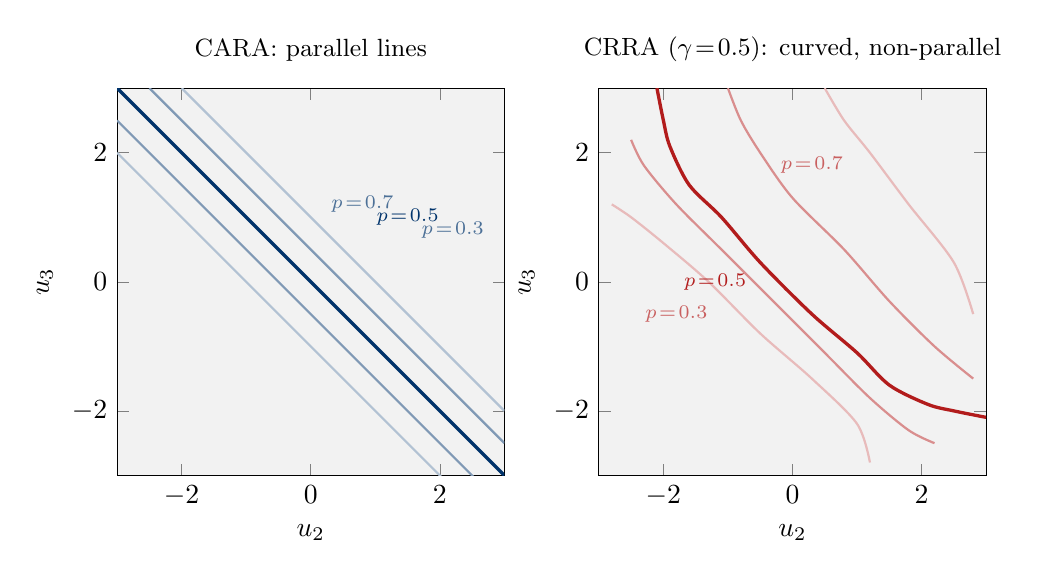
\begin{tikzpicture}
% CARA panel
\begin{axis}[
  name=cara,
  xmin=-3, xmax=3, ymin=-3, ymax=3,
  xlabel={$u_2$}, ylabel={$u_3$},
  width=6.5cm, height=6.5cm,
  axis equal image,
  title style={font=\small},
  title={CARA: parallel lines},
  axis background/.style={fill=black!5}]
% Multiple price contours — all straight, parallel
\addplot[thick,color=blue!30] coordinates {(-3,2.0)(3,-4.0)};
\addplot[thick,color=blue!50] coordinates {(-3,2.5)(3,-3.5)};
\addplot[very thick,color=blue] coordinates {(-3,3.0)(3,-3.0)};
\addplot[thick,color=blue!50] coordinates {(-2.5,3)(3,-2.5)};
\addplot[thick,color=blue!30] coordinates {(-2.0,3)(3,-2.0)};
\node[font=\scriptsize,color=blue!70] at (axis cs:2.2,0.8) {$p\!=\!0.3$};
\node[font=\scriptsize,color=blue] at (axis cs:1.5,1.0) {$p\!=\!0.5$};
\node[font=\scriptsize,color=blue!70] at (axis cs:0.8,1.2) {$p\!=\!0.7$};
\end{axis}

% CRRA panel
\begin{axis}[
  at={(cara.east)}, anchor=west, xshift=12mm,
  xmin=-3, xmax=3, ymin=-3, ymax=3,
  xlabel={$u_2$}, ylabel={$u_3$},
  width=6.5cm, height=6.5cm,
  axis equal image,
  title style={font=\small},
  title={CRRA ($\gamma\!=\!0.5$): curved, non-parallel},
  axis background/.style={fill=black!5}]
% Multiple price contours — curved, non-parallel
\addplot[thick,color=red!30,smooth,tension=0.5] coordinates {
  (-2.8,1.2)(-2.5,1.0)(-2.0,0.6)(-1.3,0.0)(-0.5,-0.8)(0.3,-1.5)(1.0,-2.2)(1.2,-2.8)};
\addplot[thick,color=red!50,smooth,tension=0.5] coordinates {
  (-2.5,2.2)(-2.3,1.8)(-1.8,1.2)(-1.1,0.5)(-0.3,-0.3)(0.5,-1.1)(1.2,-1.8)(1.8,-2.3)(2.2,-2.5)};
\addplot[very thick,color=red,smooth,tension=0.5] coordinates {
  (-2.1,3.0)(-2.0,2.5)(-1.9,2.1)(-1.6,1.5)(-1.1,1.0)(-0.5,0.3)
  (0.3,-0.5)(1.0,-1.1)(1.5,-1.6)(2.1,-1.9)(2.5,-2.0)(3.0,-2.1)};
\addplot[thick,color=red!50,smooth,tension=0.5] coordinates {
  (-1.0,3.0)(-0.8,2.5)(-0.5,2.0)(0.0,1.3)(0.8,0.5)(1.5,-0.3)(2.2,-1.0)(2.8,-1.5)};
\addplot[thick,color=red!30,smooth,tension=0.5] coordinates {
  (0.5,3.0)(0.8,2.5)(1.2,2.0)(1.8,1.2)(2.5,0.3)(2.8,-0.5)};
\node[font=\scriptsize,color=red!70] at (axis cs:-1.8,-0.5) {$p\!=\!0.3$};
\node[font=\scriptsize,color=red] at (axis cs:-1.2,0.0) {$p\!=\!0.5$};
\node[font=\scriptsize,color=red!70] at (axis cs:0.3,1.8) {$p\!=\!0.7$};
\end{axis}
\end{tikzpicture}
\end{document}
